\subsection{Visualisierungwebseite}\label{ss:visualisierung}



Durch die Kombination der SunSPOT-Sensoren mit einem kleinen Computer lässt sich das System mit einer interaktiven Visualisierung erweitern. Hierbei erhält der Computer von der SunSPOT-Basisstation Informationen über die Umgebung. Dies können beispielsweise die aufgezeichneten Vibrationen der Sensoren sein.\\
Auf dem Computer wird ein Webserver eingerichtet, der mit den erhaltenen Informationen eine Webseite erstellt, auf die der Wohnungsbesitzer zugreifen kann. Hier erhält er einen Überblick über den Status seiner Wohnung und besitzt die Möglichkeit mit dem Sicherheitssystem zu interagieren. 

\vspace{5 mm}
\begin{figure}[H] 
	\centering
	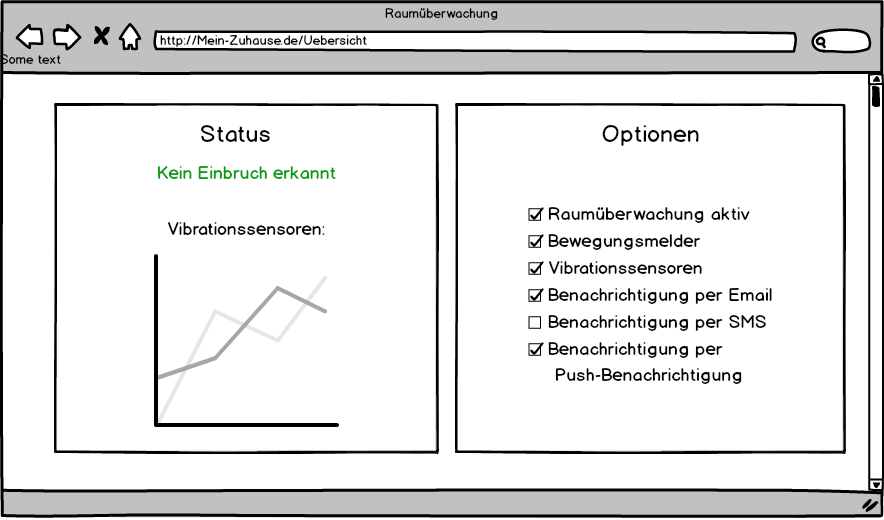
\includegraphics[scale=0.47]{Bilder/mockupwebsite}
	\caption{Mockup einer Webseite}
	\label{f:mockupwebsite}
\end{figure}

Die Umsetzung dieser Erweiterung ist mit Hilfe eines Raspberry Pis möglich. Dieser besitzt einen USB-Anschluss, über den die Basisstation der SunSPOTs angeschlossen werden kann. Zusätzlich kann sich der Raspberry Pi über Ethernet oder WLAN mit dem Internet verbinden.\\
Mithilfe der Debian-Linux Distribution Raspbian kann ein Tomcat- oder Apache Webserver aufgesetzt werden, der die Webseite des Überwachungssystems bereitstellt. Auf der Webseite kann dem Besitzer das Aktivieren sowie Deaktivieren der Überwachung oder einzelner Sensoren ermöglicht werden.

\begin{figure}[H] 
	\centering
	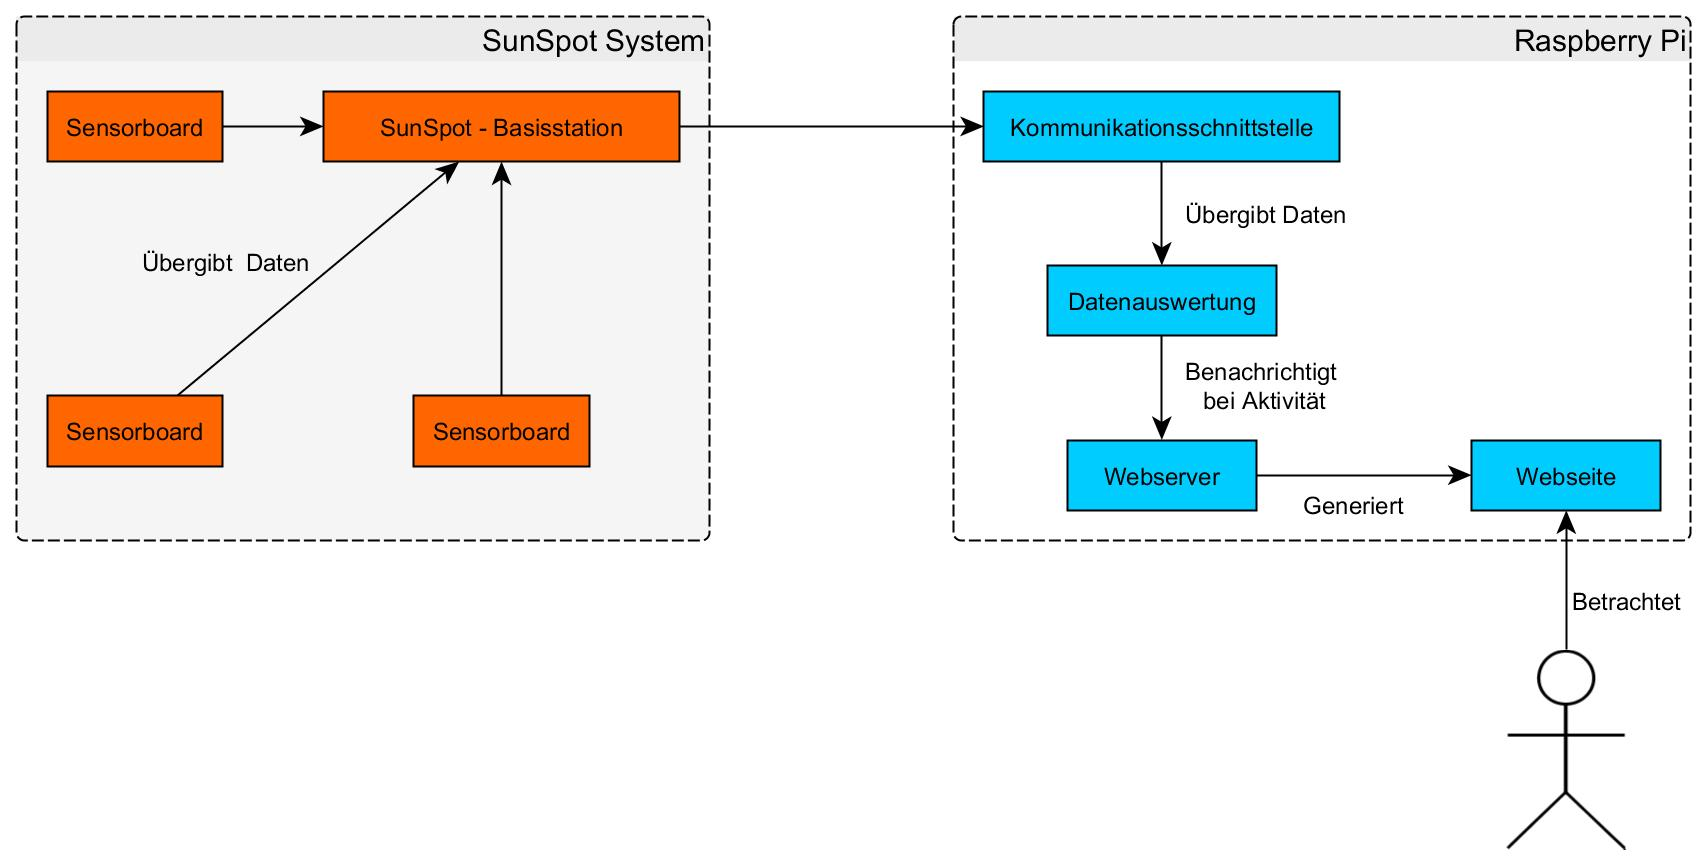
\includegraphics[scale=0.25]{Bilder/Visualisierung}
	\caption{Visualisierung mit Hilfe eines Raspberry Pis und Webserver}
	\label{f:visualisierung}
\end{figure}